\section{Time Series}

A time series, also known as discrete time signal, is a sequence of observations taken periodically in time. We can use time series to perform many tasks such as predictions of future values, behaviour analysis or information extraction. Examples of time series are audio signals, industrial instrument measures or diary finantial activity.

\begin{figure}[H]
  \centering
  % This file was created with tikzplotlib v0.10.1.
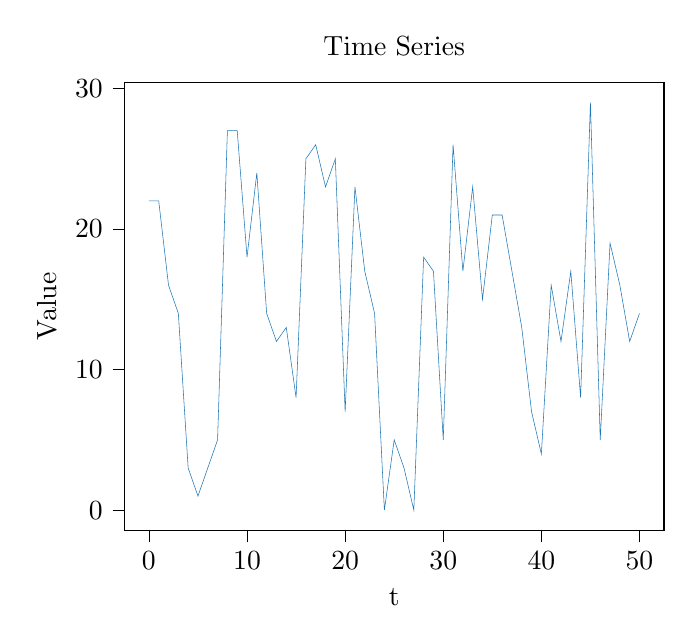
\begin{tikzpicture}

\definecolor{darkgray176}{RGB}{176,176,176}
\definecolor{steelblue31119180}{RGB}{31,119,180}

\begin{axis}[
tick align=outside,
tick pos=left,
title={Time Series},
x grid style={darkgray176},
xlabel={t},
xmin=-2.5, xmax=52.5,
xtick style={color=black},
y grid style={darkgray176},
ylabel={Value},
ymin=-1.45, ymax=30.45,
ytick style={color=black}
]
\addplot [very thin, steelblue31119180]
table {%
0 22
1 22
2 16
3 14
4 3
5 1
6 3
7 5
8 27
9 27
10 18
11 24
12 14
13 12
14 13
15 8
16 25
17 26
18 23
19 25
20 7
21 23
22 17
23 14
24 0
25 5
26 3
27 0
28 18
29 17
30 5
31 26
32 17
33 23
34 15
35 21
36 21
37 17
38 13
39 7
40 4
41 16
42 12
43 17
44 8
45 29
46 5
47 19
48 16
49 12
50 14
};
\end{axis}

\end{tikzpicture}

  \caption{Example of a random time series.}
\end{figure}
A system can be determined comparing the input and the output. We call the system a filter if it is linear and time invariant. Considering the dynamic system as a black box, we can estimate the transference function or the impulse response to taht filter.

We can also consider \textbf{multivariate} time series, where some values of the time series have an influence on the other values in different or the same time instant. We can \textbf{classify} the time series in two wide types:

\begin{itemize}
  \item Determinist: based in dynamic systems, they exploit the phisics of the generation algorithm of the time series.
        \item Stochastic: where the series are realizations of a stochastic process, which can be modelated.
\end{itemize}

In this subject, we will focus on stochastic models.

\subsection{Stochastic Models}

We can make three big considerations on the stochastic models.
\begin{itemize}
  \item Stationary models.
        \begin{ndef}
          Let \(\{X_{t}\}\) be a stochastic process and let \(F_{X}\left(x_{t_{1} + \tau}, \dots, x_{t_{n} +\tau}\right)\) represent the CDF of the \textbf{unconditional} joint distribution of \(\{X_{t}\}\) at times \(t_{1 }+ \tau,\dots, t_{n} + \tau\). Then \(\{X_{t}\}\) is strictly stationary if
          \[
            F_{X}\left( x_{t_{1} + \tau}, \dots, x_{t_{n} +\tau}\right) = F_{X}\left(X_{t_{1}},\dots,x_{t_{n}}\right)
          \]

        \end{ndef}
        However, we will use the case of \textbf{weak stationarity}, where we assume that the expectation of the stochastic process and the covariance at times \(t,t+\tau\) are constant.

        \begin{example}
          AR, MA, ARMA
        \end{example}

  \item Non stationary models, where we do not make the assumption that the average of the process is constant in time and that there is seasonality
        \begin{example}
          ARIMA, SARIMA
        \end{example}

  \item Influenced by exogenous(extern) variables. In this cases, the exogenous variable affects the model, but the model does not affect this variable.
        \begin{example}
          SARIMAX
        \end{example}
\end{itemize}

Let us introduce some \textbf{notation} for the following explanations

\begin{ndef}
  Let \(z_{t}\) be the value of the time series at instant \(t\).
  \begin{itemize}
    \item The \textbf{backward shift} operator is \(z_{t-m} = B^{m}z_{t}\)
    \item The \textbf{forward shift} operator is \(z_{t+m} = F^{m}z_{t} = B^{-m}z_{t}\)
    \item The difference or discrete gradient operator is \(\nabla z_{t} = z_{t} - z_{t-1} = (1-B)z_{t}\)
  \end{itemize}
\end{ndef}

Recall that, having a time series we can consider its \textbf{Z-transform}, that converts the discrete-time signal into a complex frequency-domain representation. In the Z-transform representation, the previously introduced notation is:
\begin{itemize}
  \item The backward shift is \(z_{t-m} = B^{m}z_{t} = Z^{-m}z_{t}\)
  \item The forward shift is \(z_{t+m} = B^{-m}z_{t} = Z^{m}z_{t}\)
        \item The difference or discrete gradient is \(\nabla z_{t} = (1-Z^{-1})z_{t}\)
\end{itemize}


\section{Linear filter based models}

The stochastic models we use are based on time series \(z_{t}\) in which sucessive values are highly dependent. In these cases, we can see that the time series is generated from a series of independependent ``shocks''.

\begin{ndef}
  Let \(a_{t} \sim \mathcal N\left(0,\sigma_{a}^{2}\right)\) be \emph{white noise} (where each \emph{shock} is related to \(a_{t}\)) which is not observed. Consider a linear filter that transforms the unobserved \(a_{t}\) to a observed time series \(z_{t}\). We say that a \textbf{linear filter model is}
  \[
    z_{t} = \mu + a_{t} + \psi_{1}a_{t-1} + \psi_{2}a_{t-2} + \dots = \mu + \psi(B)a_{t},
  \]
  where
  \[
    \psi(B) = 1 + \psi_{1}B + \psi_{2}B^{2} + \dots
  \]
  is called the \textbf{transfer function} of the filter.
\end{ndef}

\begin{figure}[H]

  \centering
  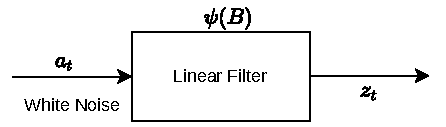
\includegraphics{Figures/LinearFilter}

\end{figure}

As we can see, we are expressing the filter in terms of a infinite sum of the coefficients \(\psi_{i}\). If there are finite coefficients of the sum is \emph{absolutely summable}, that is: \(\sum_{j = 0}^{\infty}\abs{\psi_{j}} < \infty\) or the vector of coefficients has finite \(\ell^{1}\) norm, we say that the filter is \textbf{stable} and the process \(z_{t}\) is \textbf{stationary}.

In the case where the \(\ell^{1}\) norm is not finite, our filter are non-stable and produce non-stationary series.

\subsection{Autoregressive Models (AR)}

Let us firstly consider the simplest case of linear filter. An \textbf{autoregressive model} is a linear filter where the current value of the process \(\tilde z_{t}\) is expressed as a finite sum of the previous values and a random shock \(a_{t}\).

\begin{ndef}
  Let us denote the values of a process af equally spaced times \(t,t-1,\dots\) by \(z_{t}, z_{t-1}, \dots\). Consider that the values are centered, that is \(\tilde z_{t} = z_{t} - \mu\). Then, the \textbf{autoregressive (AR) process} of \textbf{order p} is
  \begin{equation}\label{model:AR}
    \tilde z_{t} = \phi_{1}\tilde z_{t-1} + \phi_{2}\tilde z_{t-2}+ \dots  + \phi_{p}\tilde z_{t-p} + a_{t}
    \end{equation}
\end{ndef}

Note that it is called autoregressive since, if you consider \(\tilde z_{i-k}\) for \(k = 1,\dots,p\) as points, you are doing a \emph{linear regression} over the past values.\\

Now, if we define the \textbf{autoregressive operator of order p} using the backward shift operator \(B\) as:
\[
\phi(B) = 1- \phi_{1}B - \phi_{2}B^{2} - \dots - \phi_{p}B^{p},
\]
we can economically write the autoregressive model in \eqref{model:AR} as
\begin{equation}\label{model:ar:red}
  \phi(B)\tilde z_{t} = a_{t}
\end{equation}

In practice, this model has \(p+2\) unknown parameters \(\mu,\phi_{1},\dots,\phi_{p},\sigma_{a}^{2}\) which have to be estimated from the data.

\begin{nprop}
The autoregressive model is a particula case of a linear filter
\end{nprop}
\begin{proof}
  Although we will not be estrictly formal in this proof, we will give an intuition on the iterative process that has to be done.

  Consider the term \(\tilde z_{t-1}\), let us eliminate it. Recall that
  \[
    \tilde z_{t-1} = \phi_{1}\tilde z_{t-2} + \dots + \phi_{p} \tilde z_{t-p-1} + a_{t-1}.
  \]
  We can substitute this term in the expression of the AR model given in Equation \eqref{model:AR}. The same can be done for \(\tilde z_{t-2}\) and so on, to yield eventually an infinite series in the \(a\) terms.

\end{proof}

  In the case where \(p=1\), we have the AR process \(\tilde z_{t} = \phi \tilde z_{t-1} + a_{t}\). After \(m\) sucessive substitutions of \(\tilde z_{t-j} = \phi \tilde z_{t-j-1} + a_{t-j} \), with \(j = 1,\dots,m\), we obtain
  \[
    \tilde z_{t} = \phi^{m+1}\tilde z_{t-m-1}+ a_{t} + \phi a_{t-1} + \phi^{2}a_{t-2} + \dots + \phi^{m}a_{t-m}
  \]
  Now, if we take the limit \(m\to \infty\) this leads to the \emph{convergent inifinite series representation} \(\tilde z_{t} = \sum_{j=0}^{\infty}\phi^{j}a_{t-j}\), with \(\psi_{j} = \phi^{j}, j \geq 1\), provided that \(\abs{\phi} < 1\). In the general AR case,
  \[
    \phi(B) \tilde z_{t} = a_{t}
  \]
  is equivalent to
  \[
    \tilde z_{t} = \phi^{-1}(B) a_{t} = \psi(B)a_{t}, \quad \quad \psi(B) = \phi^{-1}(B) = \sum_{j=0}^{\infty}\psi_{j}B^{j}.
  \]

  AR processes can be stationary or nonstationary. From the definition, it is clear that for a AR process to be stationary, the coefficients \(\phi\) must be such that the weights \(\psi_{1},\psi_{2},\dots\) in \(\psi(B) = \phi^{-1}(B)\) form a convergent series. A \textbf{necessary requirement} for stationarity is that the autoregressive operator \(\phi(B)\), considered a polynomial in \(B\) of degree \(p\), must have all roots greater than \(1\) in absolute value.
